\documentclass[hidelinks,12pt]{article}
\usepackage[utf8]{inputenc}
\usepackage[T1]{fontenc}
%\usepackage[french]{babel}
\usepackage{times}
\usepackage{hyperref}
\usepackage{graphicx}
\usepackage{caption,graphicx,enumitem}
%\usepackage{titlesec}

%\setcounter{secnumdepth}{4}


\begin{document}

\title{Research project report}
\author{Bastien Nony, Alban Gossard\\
Institut National des Sciences Appliquées,\\
Toulouse,\\
\href{mailto:nony@etud.insa-toulouse.fr}{   \texttt{nony@etud.insa-toulouse.fr}}\\
\href{mailto:gossard@etud.insa-toulouse.fr}{   \texttt{gossard@etud.insa-toulouse.fr}}}
\date{\today}

\maketitle

\begin{abstract}
In this work we study surrogates problems for different types of modelling problem. The objective is to provide fast calculation for undetermined values. Beginning from physical equations such as Saint-Venant's, we add statistical formulas to determine the variability of the system. This study registers in the frame of geostatistics.
\end{abstract}

\newpage

\tableofcontents



\section{Objectives}
\section{Key notions}
\section{Study of 1D model}
\subsection{Presentation}
\subsection{Theoretical tools}
\subsection{Surrogate model analysis}
\subsubsection{First example : Ishigami}
\subsubsection{Garonne Model }

\paragraph{Surrogate method : kriging}
\hspace{1cm}

We compute different surrogate using different initial sample size. These surrogates were computed using a least square strategy. Figure \ref{influence_init_size_method_surrogate_kriging} gives the simulations results for the surrogate. One can observe that we obtain almost the same resultats as the initial sample size is greater than 10. As we will explain in part \ref{}, the results are quite precise but we have no information about the standard deviation of this new model and its sensibility to the parameters. Computing a surrogate with a greater number of points is fundamental to get a quantification of the error.

\begin{figure}
  \centering
  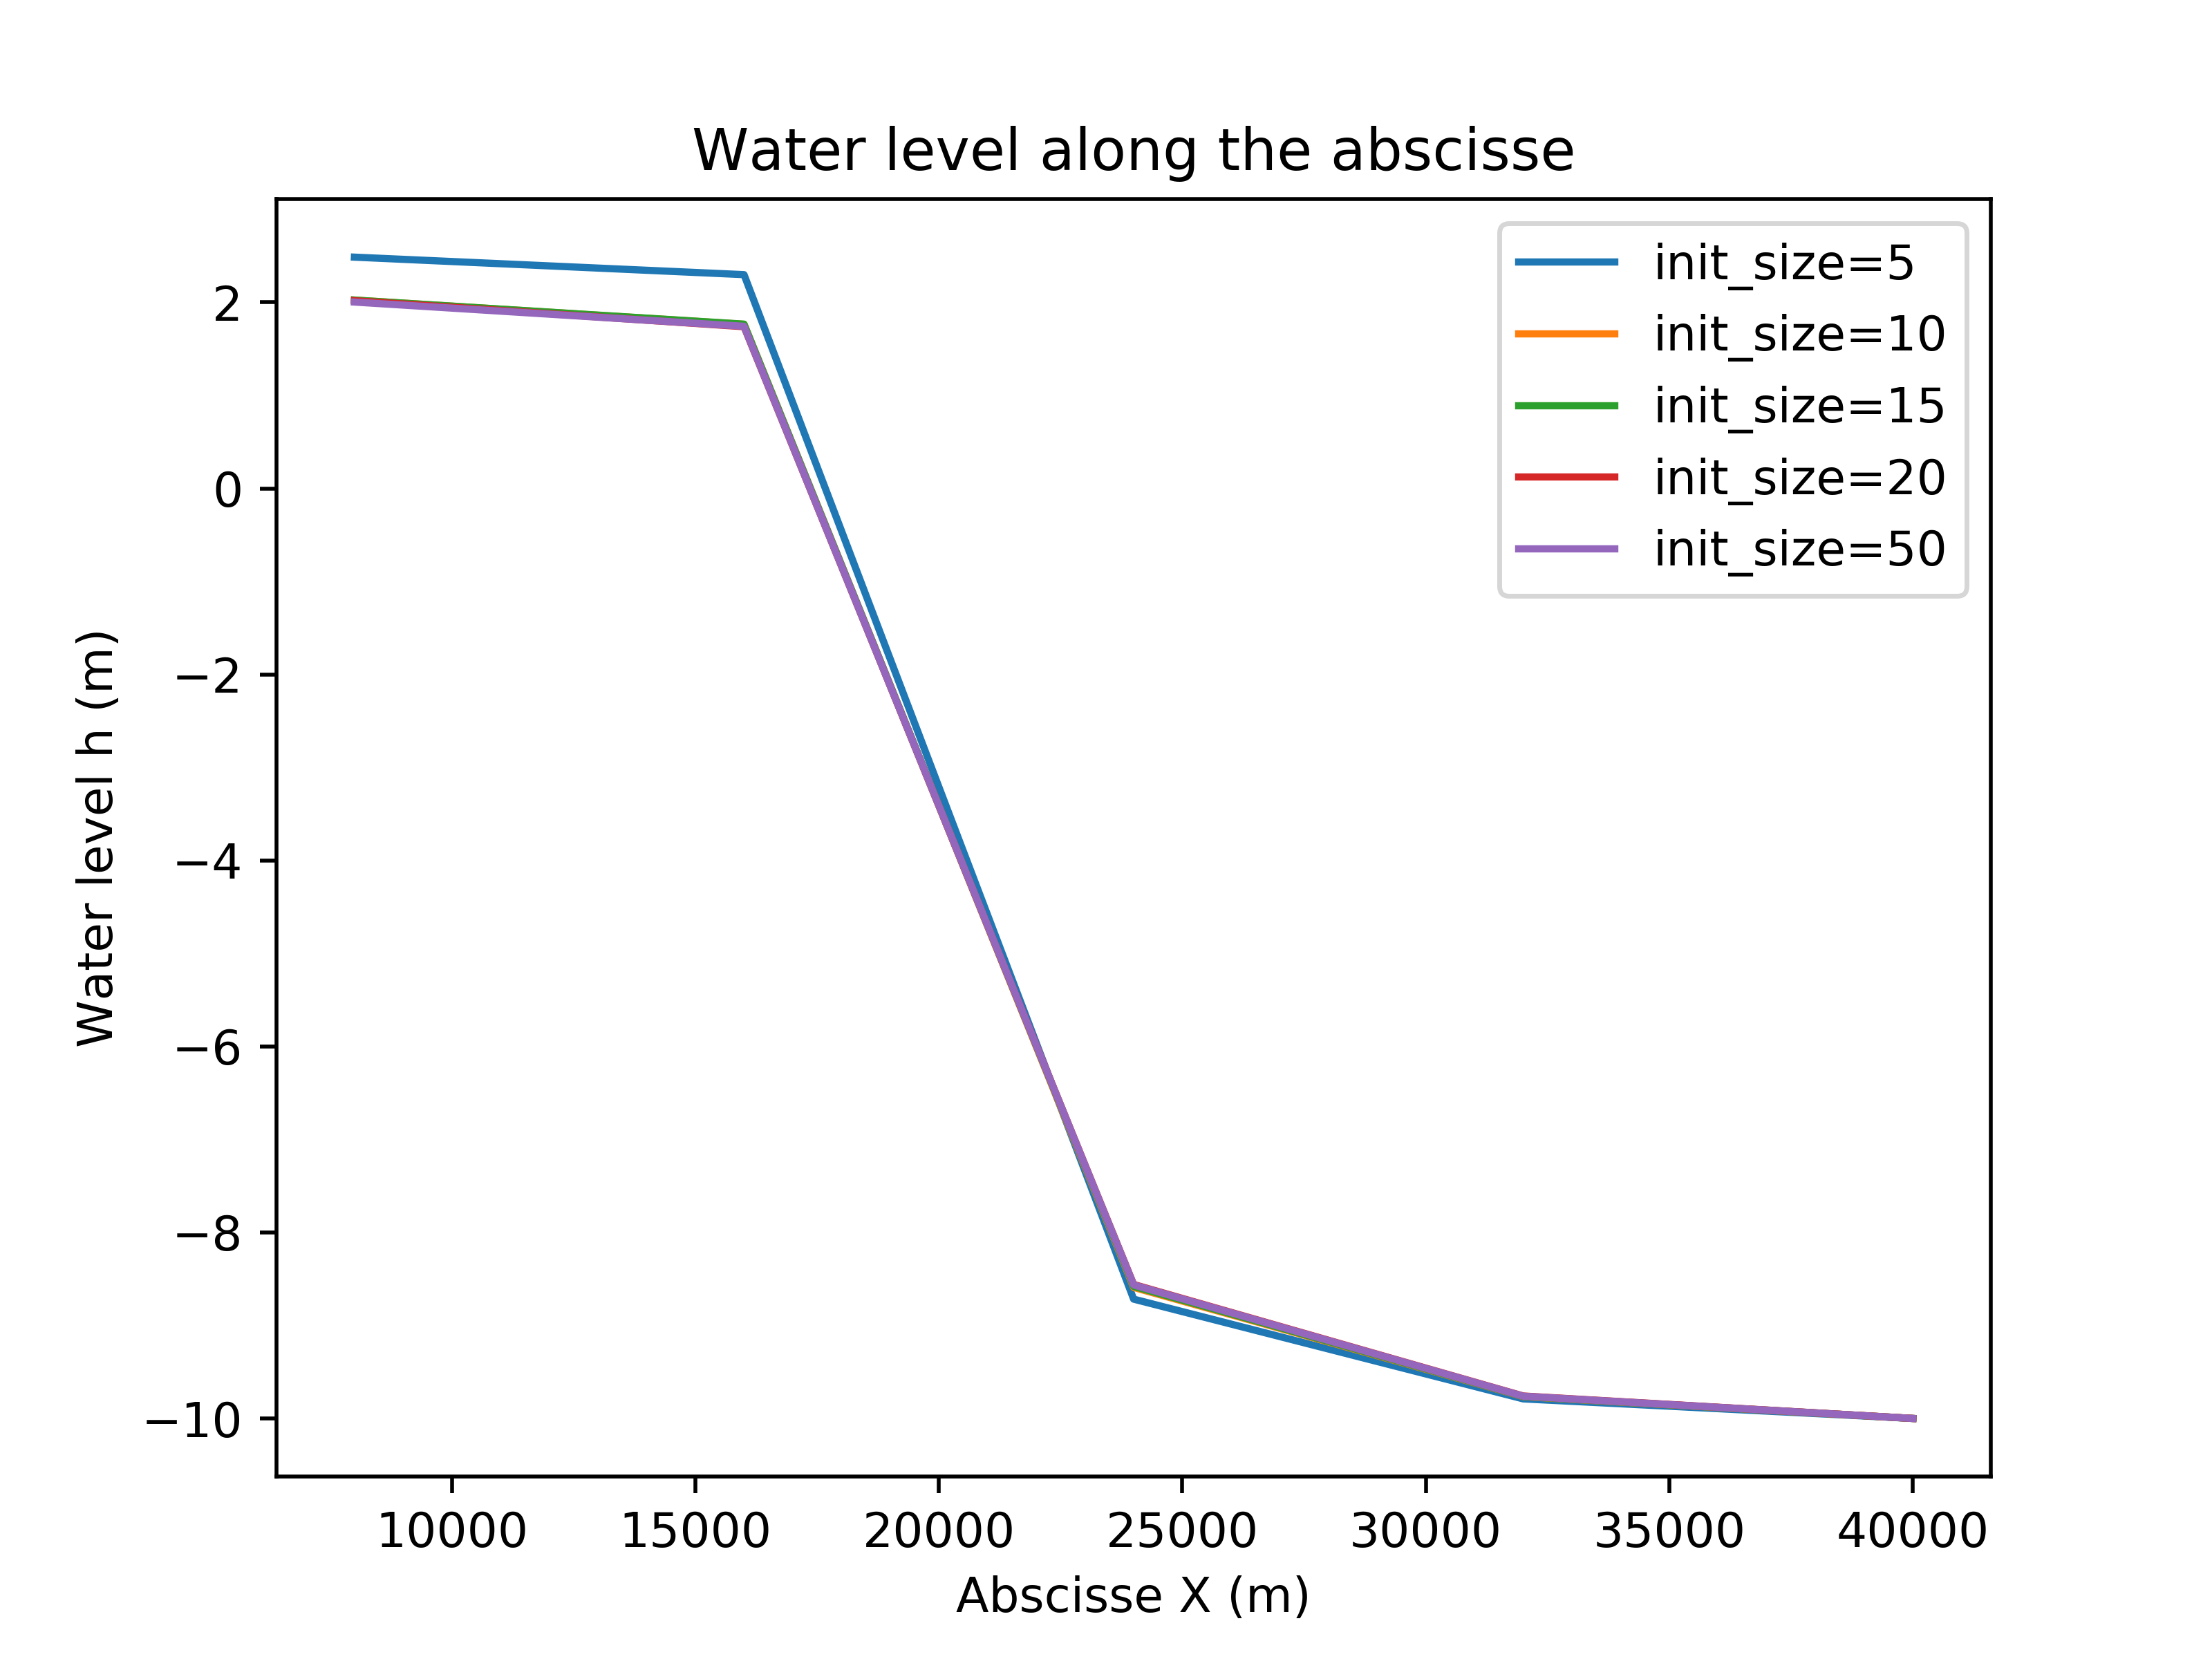
\includegraphics[width=0.8\textwidth]{images/influence_init_size_method_surrogate_kriging.png}
  \caption{Water level along the abscisse for simulations with different initial sample size using kriging method for surrogate computing.}
  	\label{influence_init_size_method_surrogate_kriging}
\end{figure}

\paragraph{Surrogate method : pc}
\hspace{1cm}

\begin{figure}
  \centering
  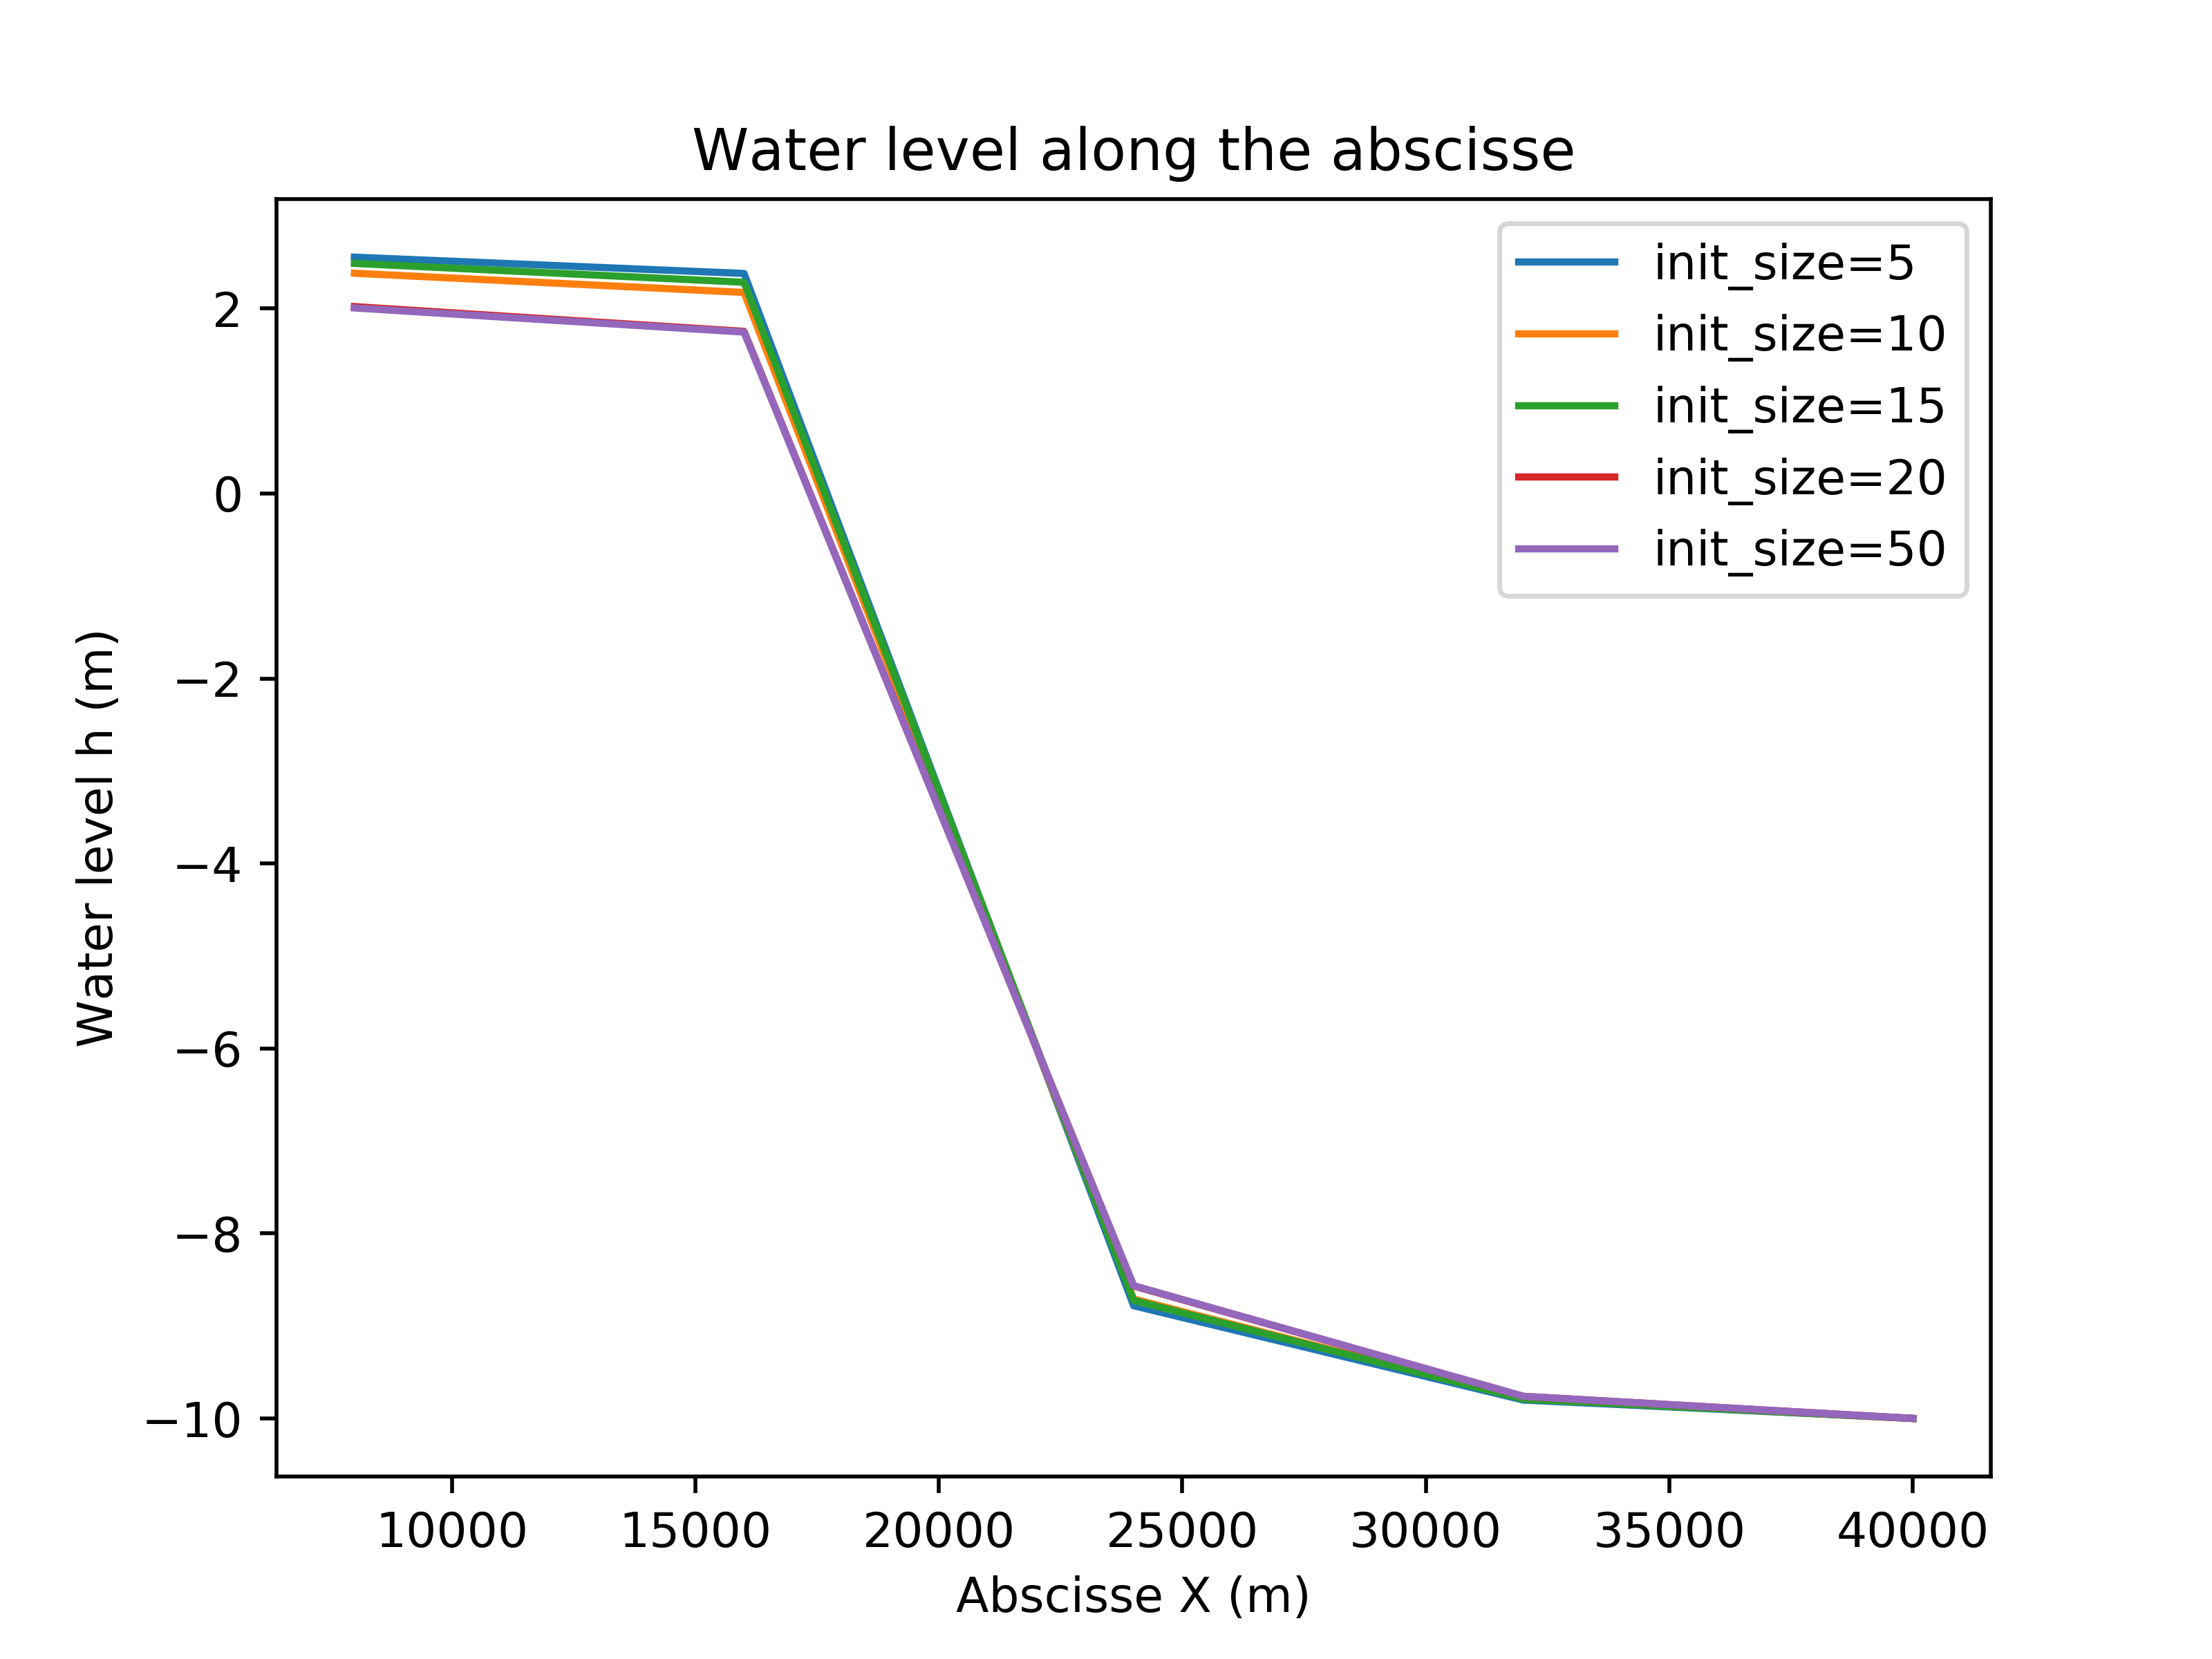
\includegraphics[width=0.8\textwidth]{images/influence_init_size_method_surrogate_pc.png}
  \caption{Water level along the abscisse for simulations with different initial sample size using pc method for surrogate computing.}
  	\label{influence_init_size_method_surrogate_pc}
\end{figure}

\begin{figure}
  \centering
  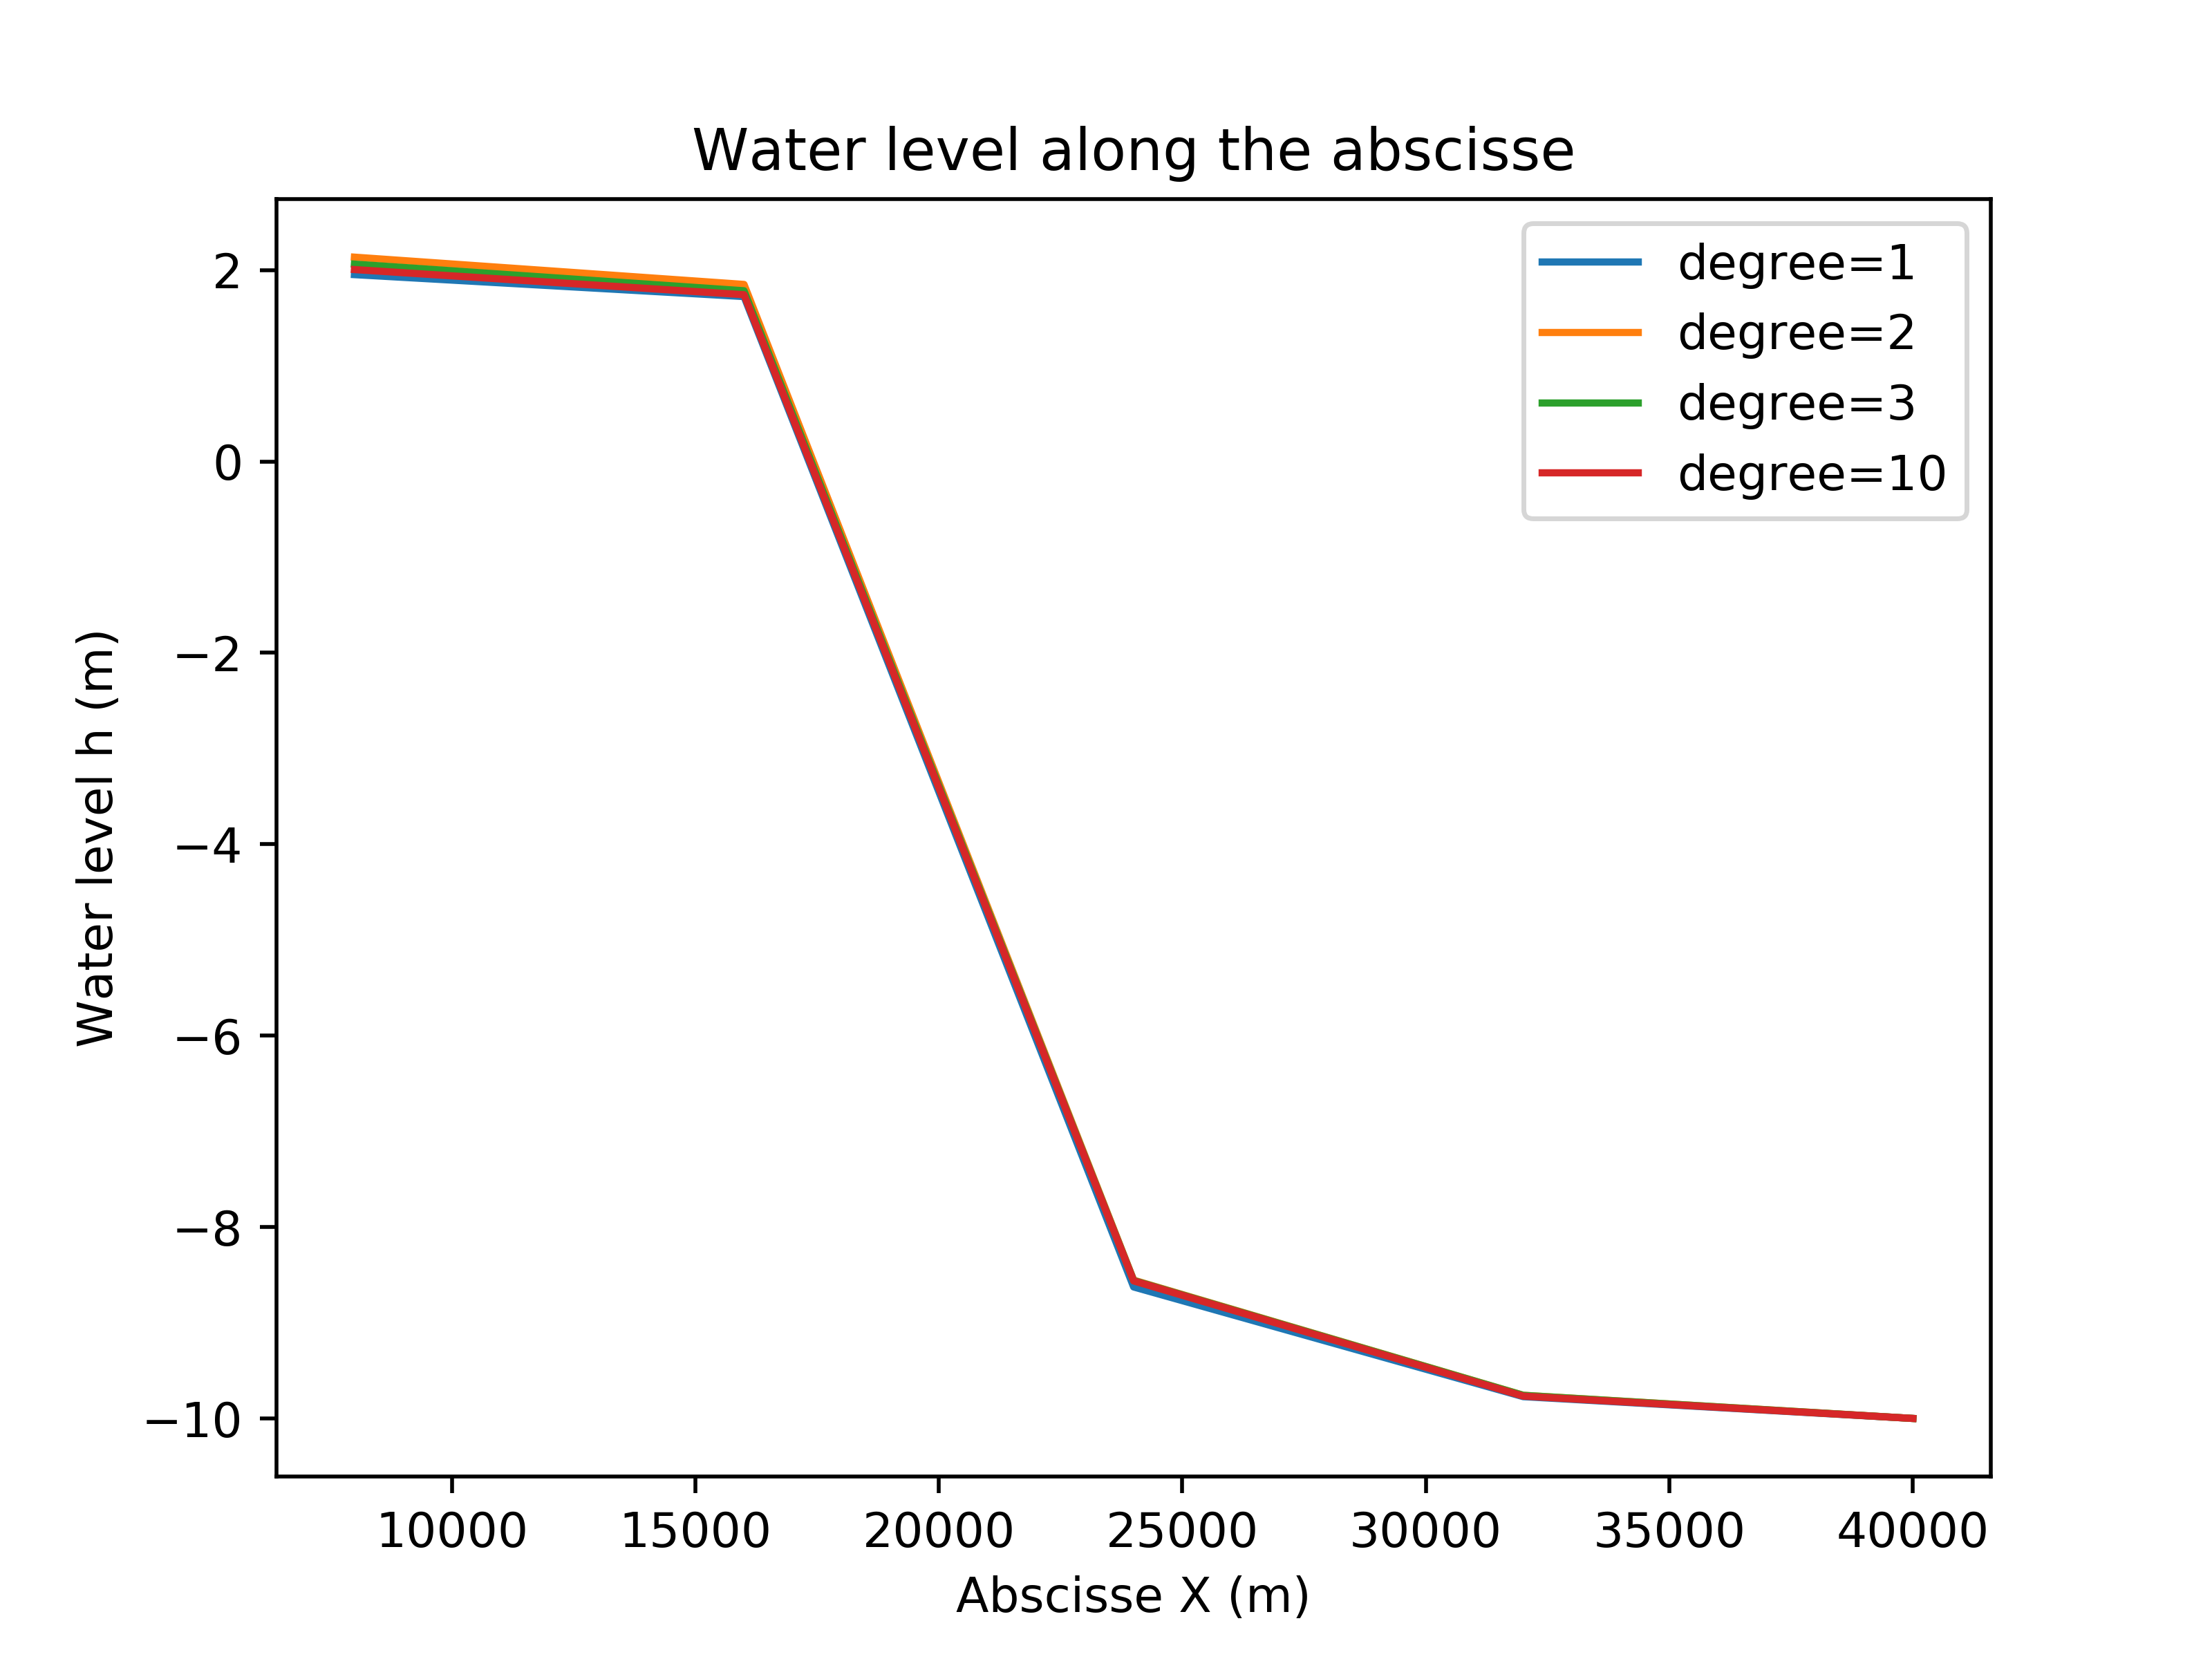
\includegraphics[width=0.8\textwidth]{images/influence_degree_method_surrogate_pc.png}
  \caption{Water level along the abscisse for simulations with different maximum pc degree.}
  	\label{influence_degree_method_surrogate_pc}
\end{figure}

\paragraph{Q2 study}
\hspace{1cm}

\begin{table}
\begin{tabular}{|c|c|}
  \hline
  Max pc degree & Q2 value \\
  \hline
  1 & 0.77805266\\
  2 & 0.95102133\\
  3 & 0.99238156\\
  4 & 0.99782457\\
  5 & 0.99813309\\
  \hline
\end{tabular}
\caption{Q2 value for different maximum pc degree using pc method for surrogate computing.}
\label{influence_degree_method_surrogate_pc_Q2}
\end{table}

\subparagraph{Distributions}
\hspace{1cm}

\begin{figure}
  \centering
  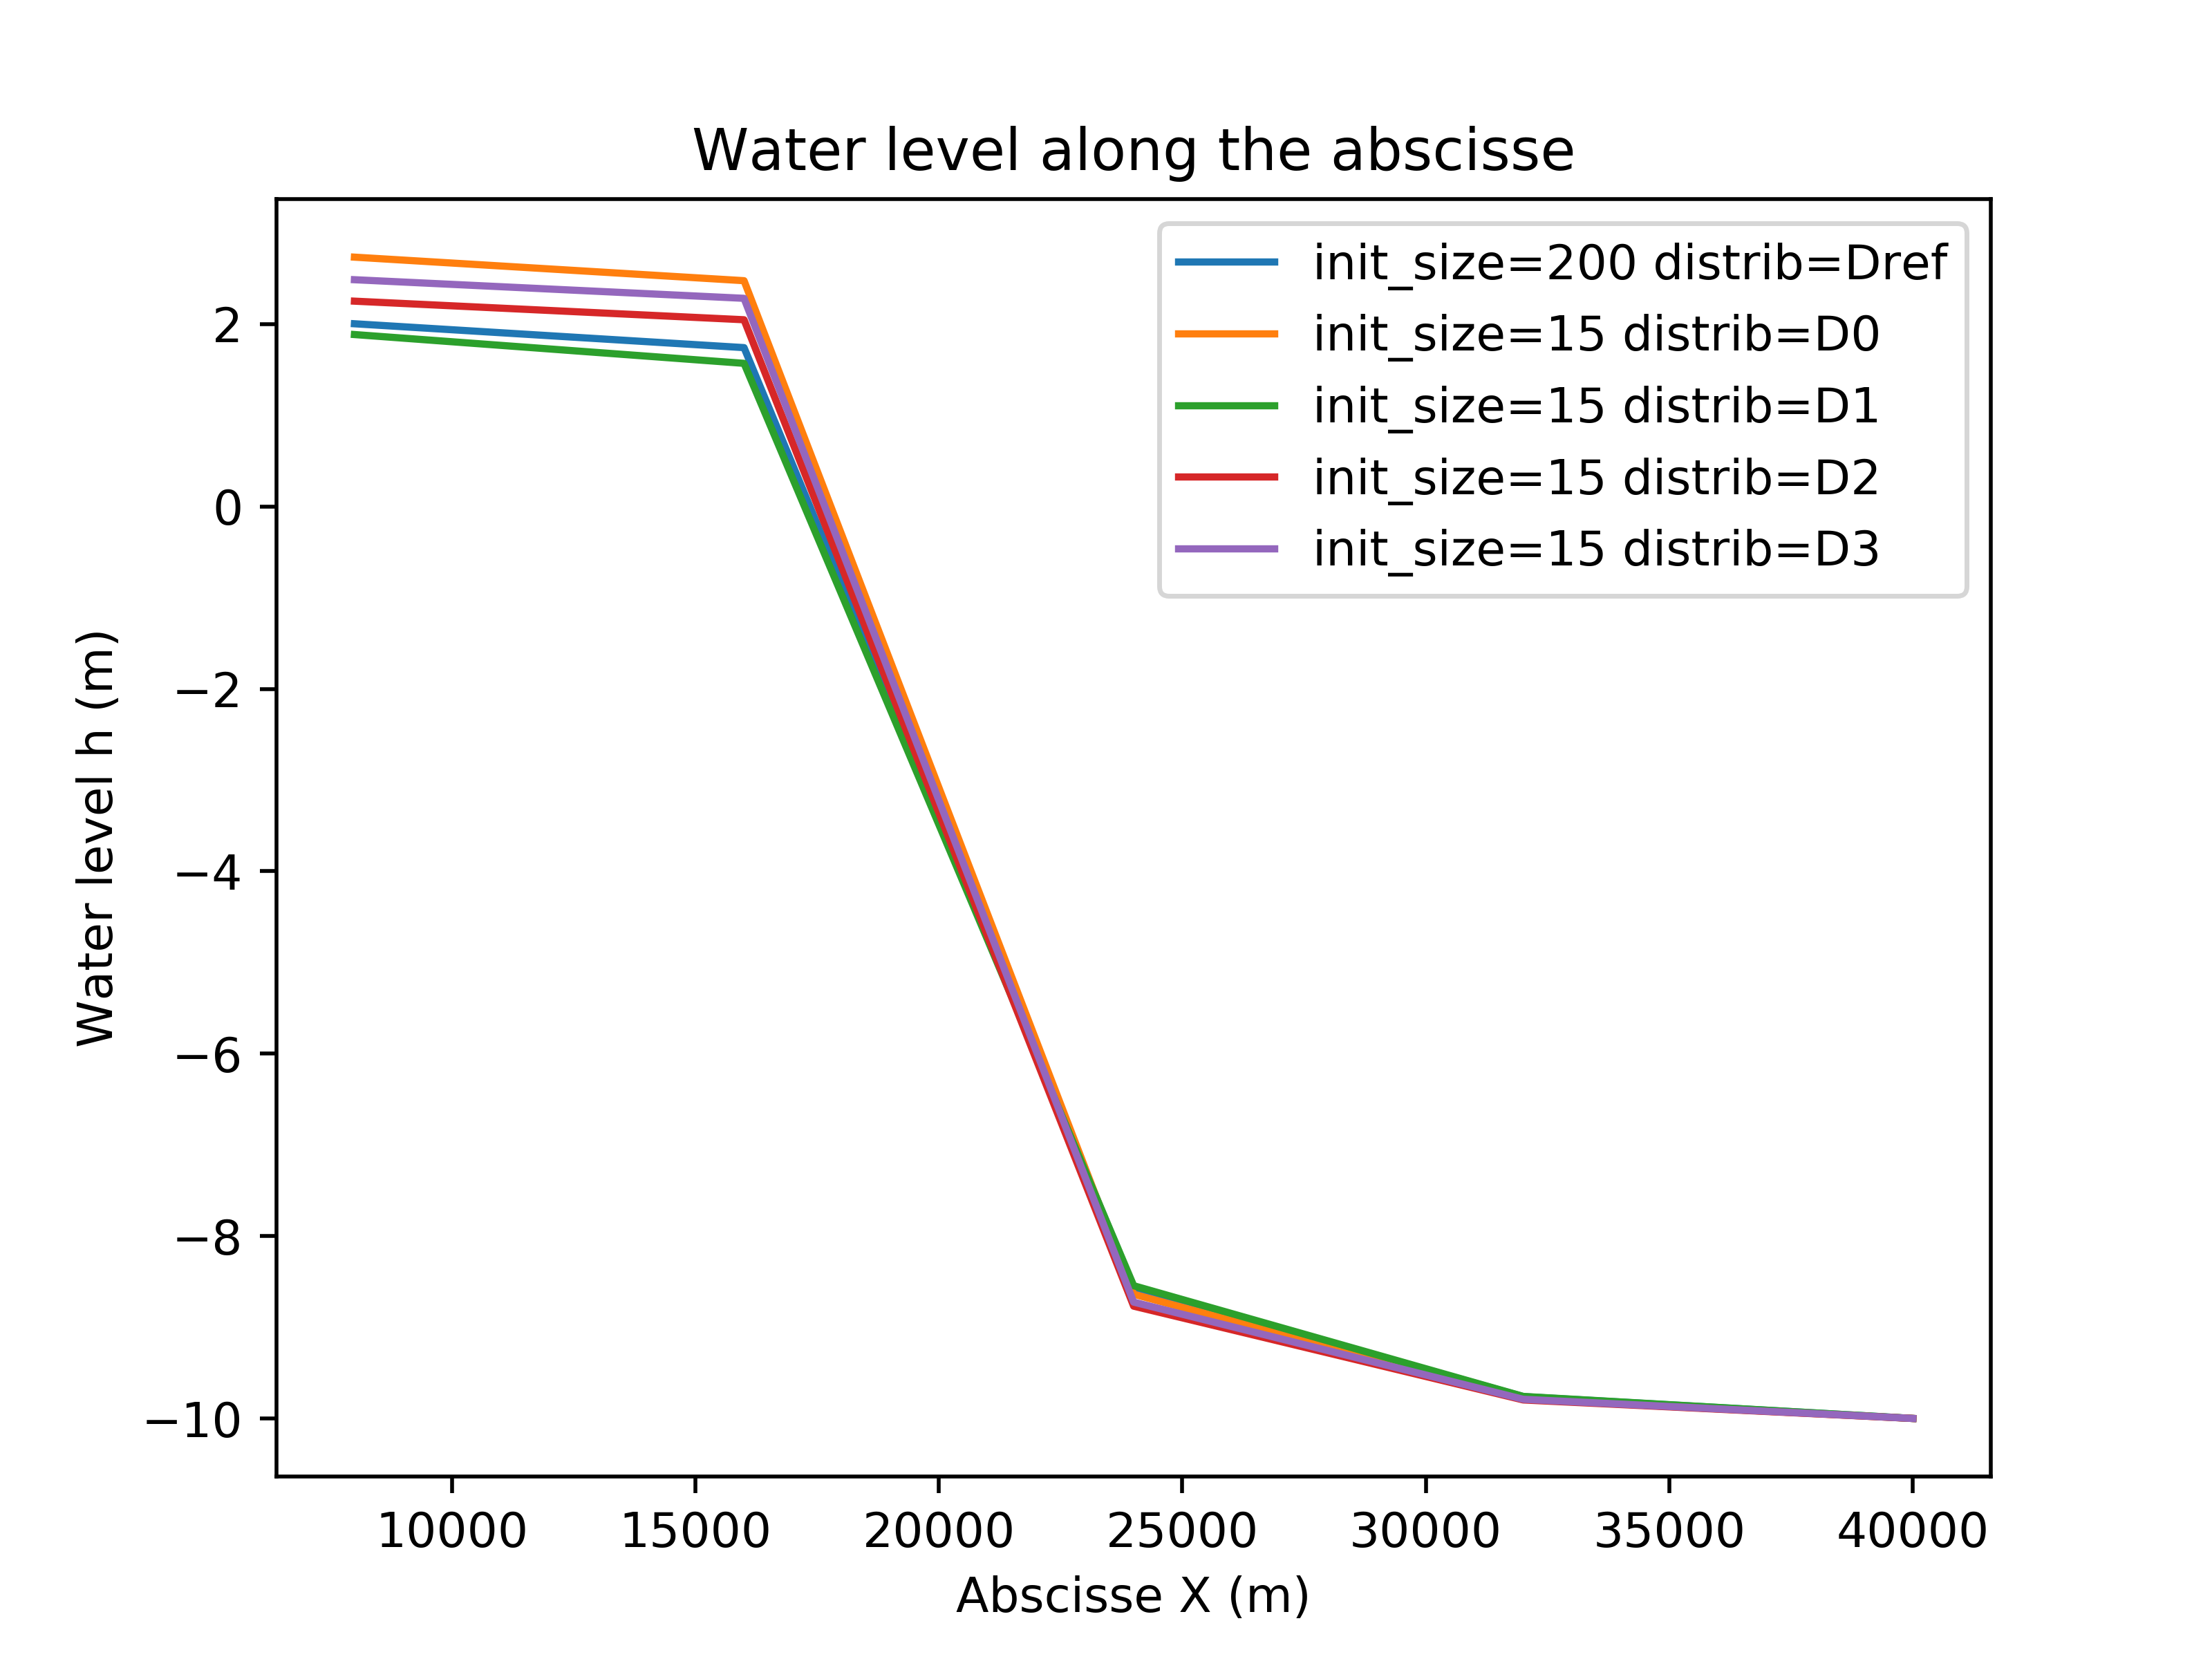
\includegraphics[width=0.8\textwidth]{images/influence_distributions_least_square.png}
  \captionsetup{singlelinecheck=off}
  \caption[]{Water level along the abscisse for simulations with different distributions for $Q$ and $K_s$ using least square strategy for surrogate computing. Distributions are the following : \begin{itemize}
  \item $D_{ref}$ : $K_s\sim BetaMuSigma(37.5, 5, 15, 60)$, $Q\sim BetaMuSigma(4035, 400, 2500, 6000)$
  \item $D_0$ : $K_s\sim Uniform(15, 60)$, $Q\sim Uniform(2500, 6000)$
  \item $D_1$ : $K_s\sim Uniform(15, 60)$, $Q\sim BetaMuSigma(4035, 400, 2500, 6000)$
  \item $D_2$ : $K_s\sim BetaMuSigma(37.5, 5, 15, 60)$, $Q\sim Uniform(2500, 6000.)$
  \item $D_3$ : $K_s\sim BetaMuSigma(37.5, 5, 15, 60)$, $Q\sim BetaMuSigma(4035, 400, 2500, 6000)$
  \end{itemize}}
  	\label{influence_distributions_least_square}
\end{figure}

One can consider that the $D_{ref}$ distribution is a good approximation of real $Q$ and $K_s$ values, meaning that we can compare different distributions with an initial sample size small to $D_{ref}$ distribution (which is computed with a high initial sample size). Figure \ref{influence_distributions_least_square} gives water level along abscisse for different sampling distributions on $Q$ and $K_s$. The distribution $D_1$ is the closest one to $D_{ref}$ suggesting we should sample the space $(Q,K_s)$ using a uniform distribution on $K_s$ and a normal one on $Q$.

\subsubsection{Michalewicz example}





\section{Annex}

%\subsection{Polynomial Chaos} ?????




\end{document}
